\chapter{Sources of ESG Risks}


\section{Cash-Flows and Discount Rate Channels}

Pastor \textit{et al.} (2021)
propose a simple one-period (period 0 and 1) overlapping generation (OLG) model 
to study the impact of climate risk on asset prices,
through both the cash-flows and discount rate channels.
To make it possible, PST (2021) splits the time 1
between $1^{-}$ and $1^{+}$, close to each other.

In the OLG model, there are two generations, $Gen-0$ and $Gen-1$.
$Gen-0$ borns at time 0 and invests in the stock of a firm.
It dies at the beginning of period 1 ($1^{-}$).
$Gen-1$ borns at the beginning of period 1 ($1^{-}$) and dies at the end of period 1 ($1^{+}$).
$Gen-0$ sells the stock to $Gen-1$ at the beginning of period 1 ($1^{-}$).
Figure~\ref{fig:fig01} shows the timeline of the model.

\begin{figure}[htbp]
    \centering
    \begin{tikzpicture}

        % Draw horizontal arrow for periods
        \draw[->] (0,0) -- (6,0) node[anchor=north] {time};
        
        % Label x-axis
        \node at (3,1) {Period};
 
        % Draw ticks and labels on x-axis
        \foreach \x in {1, 3, 5}
            \draw (\x,0.1) -- (\x,-0.1);
        \node at (2,0.5) {0};
        \node at (4,0.5) {1};


        % Draw vertical arrow for Generations
        \draw[->] (0,0) -- (0,-6) node[anchor=west] {};
 
        % Label y-axis
        \node[rotate=90] at (-1,-3) {Generation (time of birth)};
        
        \foreach \y in {-1, -3, -5}
            \draw (0.1,\y) -- (-0.1,\y);
        \node at (-0.5,-1) {0};
        \node at (-0.5,-3) {$1^{-}$};
        \node at (-0.5,-5) {$1^{+}$};

        % Draw the Gen-0
        \draw[thick] (1,-1) -- (3,-1);
        \node at (2,-0.5) {Gen-0};
        \draw[thick] (1,-3) -- (3,-3);
        \node at (2,-2.5) {Gen-0};

        % Draw the Gen-1
        \draw[thick] (3,-3) -- (5,-3);
        \node at (4,-2.5) {Gen-1};
        \draw[thick] (3,-5) -- (5,-5);
        \node at (4,-4.5) {Gen-1};
    \end{tikzpicture}
    \caption{The One-Period Overlapping Generation Model}
    \label{fig:fig01}
\end{figure}

\subsection{Cash-Flows Channel}

We denote $\pi_1$ the payoff (profit) by the
firm in period 1. It is known at $1^{-}$ (the beginning
of period 1) but received at $1^{+}$ (the end of period 1).
We denote $X_1$ this payoff per dollar 
invested in period 0: $X_1 = \frac{\pi_1}{P_0}$.

As in PST (2021), we have two sources of risk (uncertainty), $\tilde{M}$
a macroeconomic factor and $\tilde{C}$ a climate risk factor.
Those factors correspond to an unanticipated state of the world. 
For example, we could have $C$ to be a carbon tax. In that case:

\begin{equation}
    \tilde{C}_1 = C_1 - E_0(C_1)
\end{equation}

is interepreted as the difference between the expected carbon tax 
$E_0(C_1)$ and the realized carbon tax $C_1$.
These shocks occurs at $1^{-}$.

The unexpected payoff in period 1 is:

\begin{equation}
    \begin{aligned}
    X_1 - E_0(X_1) = \beta_m \tilde{M_1} + \beta_{c} \tilde{C_1} + \varepsilon_1
    \end{aligned}
\end{equation}

where $\beta_m$ and $\beta_{c}$ are the sensitivities of the payoff to the macroeconomic and climate risk factors, respectively, 
and $\varepsilon_1$ is the idiosyncratic shock to the payoff.


\begin{example}[]
\textbf{Example 1.} 
Suppose an investor in $Gen-0$ invests in a stock
with $P_0 = 100$ million USD and
expects a profit $E_0(\pi_1) = 120$ million USD.
Thus, the expected payoff 
per dollar invested at the 
beginning of the period is calculated as:

\begin{equation}
    E_0(X_1) = \frac{E_0(\pi_1)}{P_0} = \frac{120}{100} = 1.2
\end{equation}

The investor expects to earns a return of 20\% on the investment
at the end of the period.

However, two major unexpected events occur 
between period 0 and period 1:

\begin{enumerate}
    \item Macroeconomic Changes (\(\tilde{M}_1\)): The economy undergoes a downturn worse than expected, represented by \(\tilde{M}_1 = -0.05\) (a 5\% negative shock).
    \item Climate Risk (\(\tilde{C}_1\)): The government imposes a higher-than-anticipated carbon tax, leading to \(\tilde{C}_1 = 0.03\) (a 3\% additional cost).
\end{enumerate}

We assume that the idiosyncratic shock is equal to 0.

We know that the sensitivity of the firm's 
profits to economic and carbon tax shocks 
are $\beta_m = 0.5$ and $\beta_{c} = - 0.3$, 
respectively. Note that a negative $\beta_{c}$
means that higher carbon taxes reduce profits
for the firm.

The unexpected payoff is calculated as:

\[
X_1 - E_0(X_1) = (0.5 \times -0.05) + (- 0.3 \times 0.03) = -0.034
\]
Thus, the actual payoff per dollar 
invested deviates from the expected 
by -0.034, resulting 
in an actual payoff per dollar of:

\begin{equation}
    X_1 = 1.2-0.034 = 1.166
\end{equation}

In dollars terms, this translates 
into an actual end-of-period profit of:

\begin{equation}
    \pi_1 = X_1 \times P_0 = 1.166 \times 100 = 116.6
\end{equation}

instead of the expected 120 million USD.

\end{example}


The price $p_1$ is calculated at $1^{-}$ when
shocks associated with $X$ 
have been realized. Therefore, 
between $1^{-}$ and $1^{+}$, the payoff is
riskless (everything is known).
Stockholders will 
receive the payoff at $1^{+}$.
We compute the price of the stock:

\begin{equation}
    P_1 = \frac{X_1}{1 + R^e}
\end{equation}

where $R^e$ is the excess expected return 
from PST (2021):

\begin{equation}
    R^e = \mu_m \beta_m - \frac{D}{\gamma} \beta_{c}
\end{equation}

with $\gamma$ the investor risk aversion parameter,
$D$ the average investor sensitivity to climate risk,
and $\mu_m$ the expected return on the market.
As PST (2021), we assume the 
risk free rate $r_f = 0$, $\beta_m = 0$ and the investor 
risk aversion parameter $\gamma$ and the 
firm sensitivity to climate risk $\beta_{c}$
doesn't change between $Gen-0$ and $Gen-1$.
Figure~\ref{fig:fig02} shows the price of the stock 
sensitivity to $\beta_{c}$, $D$ and $\gamma$.


We assume for the moment that the average 
investor sensitivity to climate risk $D$ 
doesn't change between $Gen-0$ and $Gen-1$.
We have the payoff for $Gen-0$ at $1^{-}$:

\begin{equation}
    \begin{aligned}
    P_1 = \frac{X_1}{1 - \frac{D}{\gamma} \beta_{c}} \\
    \approx X_1 + \frac{\beta_{c}}{\gamma}D
    \end{aligned}
\end{equation}

where we have followed the approximation
from PST (2021)\footnote{
With $\rho_1 := X_1 - 1$ and $\rho_2 := \frac{\beta_{c}}{\gamma}D$,
we have:
\begin{equation}
    \begin{aligned}
        \frac{1 + \rho_1}{1 - \rho_2} = \frac{(1 + \rho_1)(1 + \rho_2)}{1 - \rho_2^2} \\
        \approx (1 + \rho_1)(1 + \rho_2) \\
        = 1 + \rho_1 + \rho_2 + \rho_1 \rho_2 \\
        \approx 1 + \rho_1 + \rho_2
    \end{aligned}
\end{equation}

where the approximation are $\rho^2_2$ and $\rho_1 \rho_2$ are small.
The assumptions are valid when $\rho_1$ and $\rho_2$ are small.
}.


Figure~\ref{fig:price} shows the price of the stock 
sensitivity to $\beta_{c}$, $D$, $\gamma$ and $X$.

\begin{figure}
    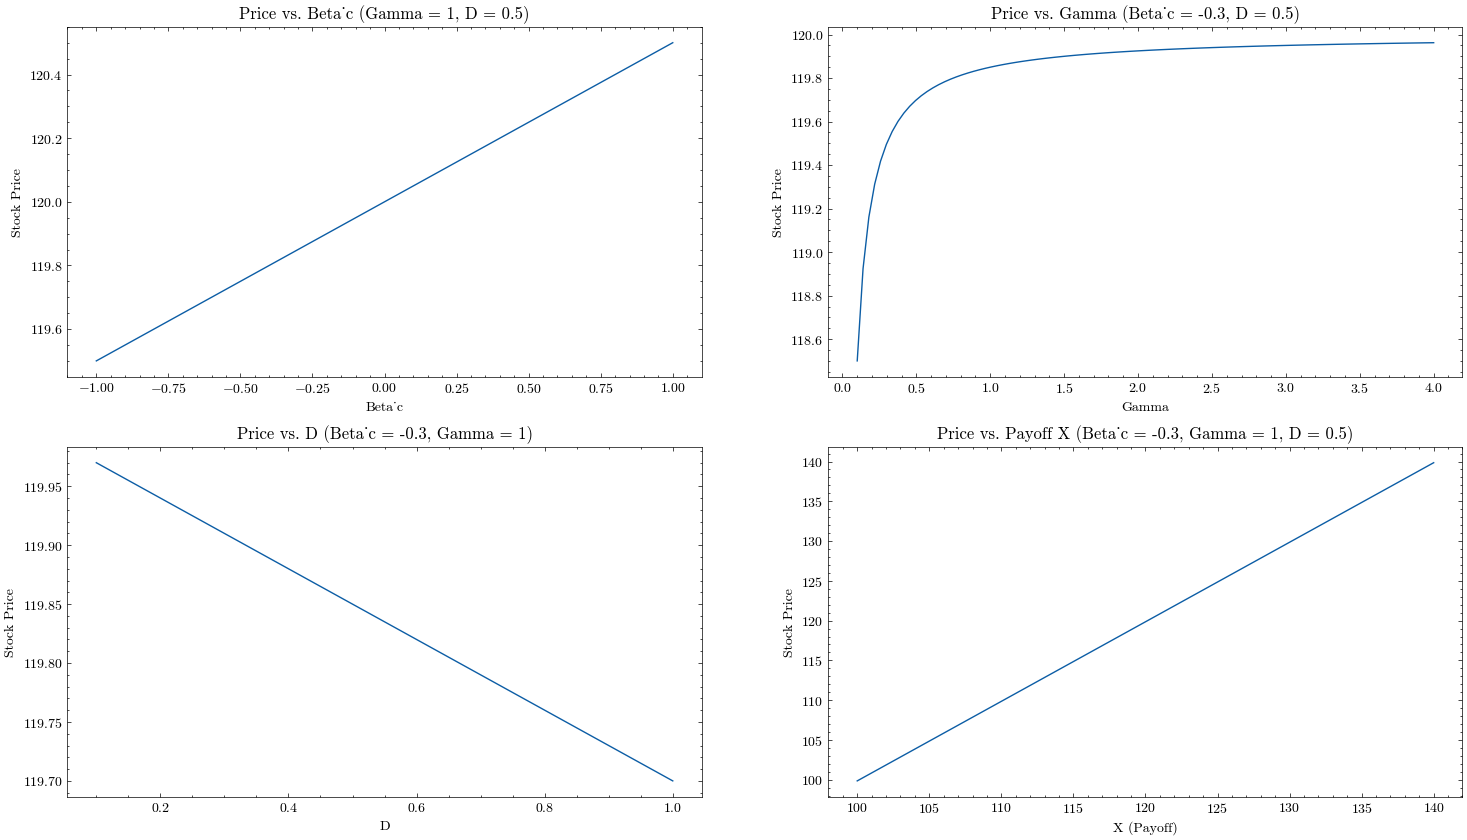
\includegraphics[width=\textwidth]{../images/chapter02/price_vs_parameters.png}
    \caption{Price of the stock as a function of $\beta_{c}$, $D$, $\gamma$ and 
    $X$}
    \label{fig:price}
\end{figure}

It's expected value when $Gen-0$ invested in period 0 was:

\begin{equation}
    E_0(P_1) = E_0(X_1) + \frac{\beta_{c}}{\gamma}D
\end{equation}

So the unexpected change in stock price 
for the $Gen-0$ is:

\begin{equation}
    \begin{aligned}
    P_1 - E_0(P_1) = X_1 + \frac{\beta_{c}}{\gamma}D - E_0(X_1) - \frac{\beta_{c}}{\gamma}D \\
    = X_1 + \frac{\beta_{c}}{\gamma}D - E_0(X_1) - \frac{\beta_{c}}{\gamma}D \\
    = X_1 - E_0(X_1) \\
    = \beta_{c} \tilde{C_1} + \varepsilon_1
    \end{aligned}
\end{equation}

\begin{example}[]
    \textbf{Example 2.} 
    Continuing our previous example, but with 
    $\beta_m = 0$. We have then 
    the unexpected loss in stock price to be: 

    \begin{equation}
        \begin{aligned}
        P_1 - E_0(P_1) = \beta_{c} \tilde{C_1} + \varepsilon_1 \\
        = -0.3 \times 0.03 + 0 = -0.009
        \end{aligned}
    \end{equation}

    With the shock $\tilde{C}_1 = 0.03$, the
    investor in $Gen-0$ will 
    suffer a loss of 0.9\% in the stock price.
    
\end{example}

\subsection{Introducing the Discount Rate Channel}

To model the discount rate channel, PST (2021)
assume that the average investor sensitivity to climate risk 
$D$ shifts unpredictably from time 0 
to time 1. 
At time $1^{-}$, $Gen-0$ sell stocks 
to $Gen-1$ at price $P_1$, which depends 
on the average sensitivity to climate risk
of $Gen-1$, $D_1$ and the payoff $X_1$.
This setting maintains single-period 
payoff uncertainty but allows risk
stemming from from climate risk to enter 
via both cashflows and discount rates 
channels.

The price $P_1$ is now:

\begin{equation}
    \begin{aligned}
    P_1 = X_1 + \frac{\beta_{c}}{\gamma}D_1
    \end{aligned}
\end{equation}

Taking the expectations:

\begin{equation}
    \begin{aligned}
    E_0(P_1) = X_1 + \frac{\beta_{c}}{\gamma}E_0(D_1) 
    \end{aligned}
\end{equation}

The unexpected loss in stock price is now:

\begin{equation}
    \begin{aligned}
    P_1 - E_0(P_1) = X_1 + \frac{\beta_{c}}{\gamma}D_1 - E_0(\tilde{X_1}) - \frac{\beta_{c}}{\gamma}E_0(D_1) \\
    = X_1 - E_0(X_1) + \frac{\beta_{c}}{\gamma}(D_1 - E_0(D_1)) \\
    = \beta_{c} \tilde{C_1} + \varepsilon_1 + \frac{\beta_{c}}{\gamma}(D_1 - E_0(D_1)) \\
    = \beta_{c}(\tilde{C_1} + \frac{1}{\gamma}(D_1 - E_0(D_1))) + \varepsilon_1
    \end{aligned}
\end{equation}

